\chapter{Background}
\label{ch:background}

Formal methods are a specific type of mathematical notation which is based on the techniques of the specification, verification and development of software and hardware systems \cite{whatareformalmethods}. Since our thesis presents \gls{zmath} we go right to the beginning of the framework, to describe how mathematical notation came about. Then we describe the original MathLang framework (the framework which \gls{zmath} is an adaptation of) and then give the reader an idea of other formal methods and languages. In the next section we wish to describe what is the language of Z and give more details of it's syntax and semantics. We then highlight other proving techniques which have been done for maths, formal methods and Z.

\section{Mathematical Notations}

Computer science (and thus computer systems) have evolved from basic mathematics. We can say that formal specification writers are practising mathematicians as they write system specifications in a formal manner. Therefore we must start right at the beginning at the foundation of mathematical notation.

\subsection{Right from the beginning}
\label{subsec:rftb}

The relationship between mathematical reasoning and practising mathematicians started out early on during the ancient Greeks where logic was already being studied. Reasoning in logic was used for just about anything not just mathematics such as law, medicine and farming. This very early form of mathematics made very famous discoveries such as Aristotles logic \cite{aristotle}, Euclid's geometry \cite{euclid} and Leibniz Calculus \cite{leibniz}.

Further on in the 1800's, Frege wrote \emph{Die Grundlagen der Arithmetik} \cite{frege} and other works where he noted that mathematics is a branch of logic. In this works, he began building a solid foundation for mathematics. This early foundation along with Cantors set theory \cite{cantor} was argued to be incosistant and thus Russel found a pardox in this work.

In the late 19th century and beginning of 20th century, Russell \& Whitehead \cite{whitehead1912principia} started to form a basis for mathematical notation. Their three volume work describes a set of rules from which all mathematical truths could be proven. In these early stages the authors try to dervive all maths from logic. This ambitious project was the first stepping stone in collaborating all mathematics under one notation.

Further to Russell \& Whitehead's work, Bourbanki \footnote{A name given to a collective of mathematicians} wrote a series of books beginning n the 1935's with the aim of grounding mathematics. Their main works is included in the Elements of Mathematics series \cite{opac-b1128208} which does not need any special of knowledge of mathematics. It describes mathematics from the very beginning and goes through core mathematical concepts such as set theory, algebra, function etc and gives complete proofs for these concepts.

Adding to Russell's work, Zermelo introduced an acclimatisation of set theory which was later extended by Frankel and Skolem to form ZF set theory \cite{zfc}. This new theory is what we will later see the Z notation is based on and the notation this thesis checks the correctness of.

\subsection{Computerisation of Maths and Proof Systems}

In the 21st century, a great area of research is how use, store and support this mathematical knowledge. Since automation has become more and more used, mathematicians have looked into ways in which they can use computers to reason about and provide services to mathematics. This would include all areas of mathematics, such as logic, mechanics and software specifications. Mathematical knowedge can be represent in lots of different ways including the following:

\begin{itemize}
\item One can typeset mathematics into a computer using a system such as \LaTeX{} \cite{latex} . These systems can edit and format mathematical knowledge so that it can be stored or printed. These systems provide good visual appearance and thus can be used for storing and archiving ones documents. Even Z specification, have their own package for \LaTeX{} and thus the structure of the specification can be represented both formally and informally. However, it is difficult to represent the logical structure of mathematical formulas and the logical structure of mathematics is embedded in natural language. Therefore, there isn't a lot of support for checking the correctness of general mathematics represented in the system (Z specifications on their own can be checked but this is discussed further in section \ref{subsec:provingSystemsForZ}).

\item Systems such as proof assistants (e.g. Isabelle \cite{isabelle}, Coq \cite{coq} and ProofPower-Z \cite{pp}) and automated theorem provers (e.g. Boyer-Moore, Otter) and jointly called proof systems. Proof systems each provide a formal language for writing mathematics. Early work on proof systems was done by De Bruijn when he worked on the AutoMath \cite{selectedautomath} project. AutoMath (automating mathematics) was the first attempt to digitize and formally prove mathematics which was assisted by a computer. AutoMath is described as a language for formalising mathematical texts and for automating the validation of mathematics. The AutoMath project is what brought uniform notations and automated proof together.

Further to this work, there has been many other proof systems implemented to implement and check mathematics for total correctness. It is possible to access the semantics of mathematics in these systems. However, with these proof systems, a user must choose a specific proof system and one of these have their advantages and disadvantages. Also, each of these proof systems also take quite some time to learn. There is much documentation on some of these systems (e.g. Isabelle) and some are very well supported. But this in turn can be a downfall, as there is so much documentation, it is difficult to know how much one must learn and where to start. The best way of learning one of these system is from someone who already is an expert in the chosen proof system. A lot of the proof systems use proof tactics to constructs proofs and make them smaller, however to prove certain properties in a proof system, one can use various tactics to get to the same goal and may sometimes be difficult to find which tactic is best to use.

With these disadvantages many academic and industrial mathematicians do not generally use the mathematics written in the language of the proof system and usually are not willing to spend the time to check the correctness of their own work in this system.

\item There also exists semantical oriented document representations like OpenMath \cite{openmath} and OMDoc \cite{omdoc}. These systems are better than the typesetting systems such as \LaTeX{} to produce readable and printable version of the mathematical knowledge written. Some aspects of the semantics of the mathematics can be represented in these type systems. However, when using these systems it is difficult to control the presentation and therefore a typesetting system is more likely to be used. Like the typesetting system, systems like OMDoc also have difficult reading the logical structure of mathematics embedded in the natural language of the text. Systems like OMDoc can associate symbolic formulas with chunks of natural language text, however these chunks can not be seen by the computer and thus can not be checked if it is correct.

Another disadvantage is that although there is support for the semantics of the mathematics, these systems can not support the semantics in terms of logical foundations for mathematics (unlike proof systems).
\end{itemize}


\subsection{Conclusion}

In summary the \gls{math} framework has been developed to be used as a bridge between the categories mentioned above as a way to represent and automatically check mathematical knowledge. Since the Z notation has stemmed from the origins of mathematics and industry is starting to use formal methods in there system development we have chosen to adapt the \gls{math} framework to accommodate Z specification and have developed a set of tools to do so.

\section{MathLang for mathematics}
\label{sec:mathlangbackground}

\Gls{math} originally started in 2000. It's original goals was to allow gradual \gls{computerise} and \gls{formalise} of mathematical texts.

MathLang is not a system for proof verification but a framework to computerise and translate information (such as mathematical text) into a form on which proof checkers can operate.

The MathLang framework provides extra features supporting more rigour to translation of the common mathematical language. One can define further levels of translations into more semantically and logically complete versions. This gradual computerisation method should be more accessible than direct formalisation, because a number of first levels do nor require any particular expertise in formalisation.

So far Mathlang has given alternative and complete paths which transform mathematical texts into new computerised and formalised versions. Dividing the formalisation of mathematical texts into a number of different stages was first proposed by N.G. de Bruijn to relate common mathematical language to his Mathematical Vernacular \cite{mv} and his proof checking system Automath.

\subsection{Overview and Goals}

The MathLang Framework instructs the computerisation process to be broken up into a number of levels called \textbf{aspects}. Each aspect can be worked out independently, simultaneously or sequentially without prior knowledge of another aspect. The current MathLang Framework contains three well-developed aspects, the \gls{cga}, the \gls{tsa} and the \gls{dra}, and has further aspects such as the Formal Proof Sketch.

\begin{figure}[H]
\begin{center}
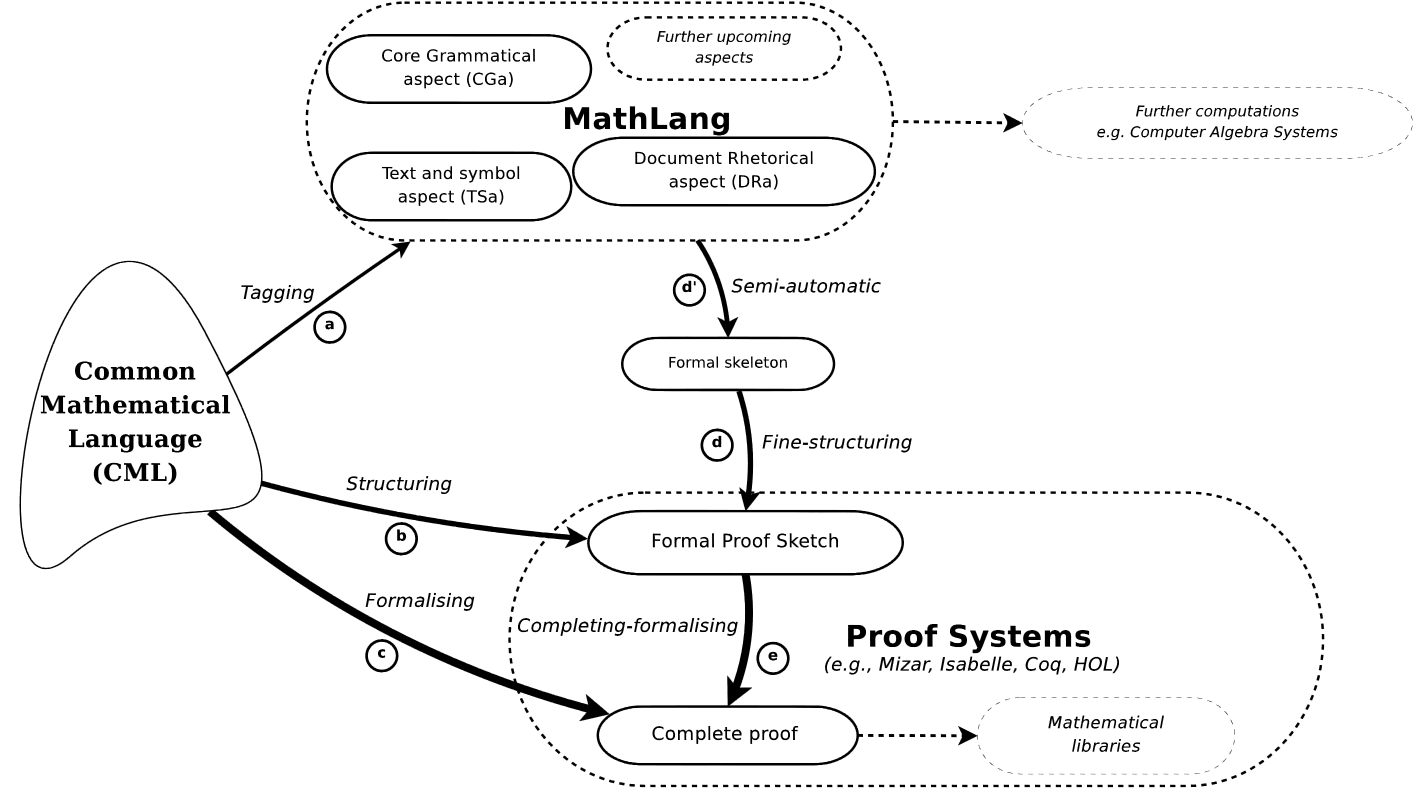
\includegraphics[scale=0.255]{Figures/Background/mathlang.png}
\end{center}
\caption{The MathLang approach to computerisation/formalisation \cite{mathintomizar}\label{fig:mathlang}}
\end{figure}

Figure \ref{fig:mathlang} shows the overall situation of work in the current MathLang Framework.
The labelled arrows show the computerisation paths from the common mathematical language to any proof system. 
The width of the arrow representing each path segment increases according to the expertise required. The level of expertise needed to computerise a CML text straight into a complete proof is very high, however the level of expertise is much smaller by using the \gls{math} framework to help form a formal skeleton and then into a complete proof. The dashed arrows illustrate further computerisation that one can envision.


\subsection{Detailed information on CGa}
\label{subsec:cga}
The current \gls{cga} in MathLang uses a finite set of grammatical \textit{categories} to identify the 
structure and common concepts used in mathematical texts. The aims of the \gls{cga} is to make explicit 
the grammatical role played by the elements of mathematical texts and to allow the validation of the grammatical and reasoning 
structure within the \gls{cga} encoding in a mathematical text. The \gls{cga} checks for grammatical correctness and finds errors like 
an identifier being used without and prior introduction or the wrong number of arguments being given to a function \cite{krzysztofphd}.

------------------------------------------

\begin{itemize}
\item Reference Zenglars quote

\item Weak type theory into CGa

\end{itemize}

\subsection{Detailed information on DRa}
\label{subsec:dra}

The Document Rhetorical aspects checks that the correctness of the reasoning in the mathematical document is correct and that there are no loops. The \gls{dra} mark-up system is simple and more concentrated on the narrative structure of the mathematical documents whereas other previous systems (such as DocBook \footnote{http://www.docbook.org}, Text Encoding Initiative \footnote{http://www.tei-c.org/index.xml}, OMDoc \footnote{http://www.omdoc.org}) were more concentrated on  the subtleties of the documents. It is used to describe and annotate chunks of texts according to their narrative role played within the document \cite{krzysztofphd}. Using the \gls{dra} annotation system we can capture the role that a chunk of text imposes on the rest of the document or on another chunk of text. This leads to generating dependency graphs which play an important role on mathematical knowledge representation. With these graphs, the reader can easily find their own way while reading the original text without the need to understand all of its subtleties. Processing \gls{dra} annotations can flag problems such as circular reasoning and poorly-supported theorems.
--------------------------------------------------------

\begin{itemize}
\item relations

\item instances

\item Dependency and goto graph
\end{itemize}

\subsection{Detailed information on skeletons}

\begin{itemize}
\item General Proof Skeleton

\item Half baked proof

\item Filled in skeleton
\end{itemize}

\subsection{information on TSa}
\label{subsec:tsa}

The \gls{tsa} builds the bridge between a mathematical text and its grammatical interpretation. The \gls{tsa} is a way of rewriting parts of the text so they have the same meaning. For example some mathematicians may prefer to write "a=b and b=c and c=d", others may prefer "a=b, b=c, c=d" and some others may prefer "a=b=c=d". As you can see all these methods of writing have the same meaning however some symbols are different. The \gls{tsa} annotates each expression in the text with a string of words or symbols which aim to act as the mathematical representation of which this expression is. This allows everything in the text to be uniform.

\subsection{A full worked examples in mathlang}

show step by step translation of mathematical text into isabelle from laamars phd thesis.

\subsection{Conclusion}

\section{Formal Methods and Languages}
\label{sec:formalmethodsandformallanguages}

Formal methods are usually used to assist in formalising in a variety of texts including systems, software and even language itself.

\begin{defin}[Formal Language]
A language designed for use in situations in which natural language is unsuitable, as for example in mathematics, logic, or computer programming.\footnote{www.dictionary.com/browse/formal-language}
\end{defin}

\begin{defin}[Formal Specification]
The specification of a program's properties in a language defined by a mathematical logic.\footnote{www.wiki.c2.com/?FormalSpecification}
\end{defin}

\begin{defin}[Formal methods]
Mathematical approaches to software and system development which support the rigorous specification, design and verification of computer systems.\footnote{www.fmeurope.org/?page\_id=2}
\end{defin}

Formal methods are mathematical approaches to software and system development which support the rigorous specification, design and verification of computer systems \cite{fmeurope}. Specifications are a collection of statements describing how a proposed system should act and function. Formal specifications use notations with defined mathematical meanings to describe systems with precision and no ambiguity. The properties of these specifications can then be worked out with more confidence and can be described to the customers and other stakeholders. This can uncover bugs in the stated requirements which may not have found in a natural language specification. With this, a more complete requirements validation can take place earlier in the development life-cycle and thus save costs and time of the overall project. The rigor using formal methods eliminates design errors earlier and results in substantially redecued time \cite{benefitsofform}. 

\subsection{A brief history of formal methods}

The first known formal language is thought to be used by Frege in his Begriffsschift (1879), Begriffschift meaning `concept of writing' described as `formal language of pure thoguht'. Frege formalised propositional logic as an axiomatic system.

Formal methods then grew in the following:

\begin{itemize}
\item 1940's, Alan Turing annotated the properties of program states to simplify the logical analysis of sequential programs

\item 1960's Floyd, Hoare and Naur recommended using axiomatic techniques to prove programs meet their specification.

\item 1970's Dijkstra used formal caluculus to aid development of non-deterinist programs
\end{itemize}

Formal methods are used today are just as important as when they were used before. Formal methods have a large presence in academia and have also made their way into various industries to prevent design flaws in high integrity systems. Previous desing errors have been found in systems such as the Therac-25 machine, which was used for radiation therapy produced by Atomic Energy of Canada Limited in 1982. It was involved in multiple incidents in which patients were give massive overdoses of radiation \cite{baase2003gift}. Another major fault which led to disastrous results was NASA’s Checkout Launch and Control System (CLCS) cancelled 9/2002 \footnote{www.spaceref.com/news/viewnews.html?id=475}.

\subsection{Types of formal methods}


Today there are many different types of formal methods used both in industry and academia. Specification languages are expressive languages with general proof methods, such as VDM, Z, B. Another type of formal method could be program correctness proofs which associates logical inference rules with programming syntax, e.g. Hoare triples and Gries Methodolgy.There may also be model based approaches to formal methods, which are domain specific languages with precise algorithms for correctness proofs, e.g. Temporal logic \cite{uwa}, Fuzzy logic.  

Formal methods are used to precisley communicate specifications and the function of programs. They are also used to ensure the correctness of systems particularly safety critical systems.

Formal methods have been a success in a variety of projects. For example, in the Sholis project \cite{sholis}, using a formal specification was most effective for fault finding, therefore if the specifications are correct, then the program implemented should then in turn contain less errors if it follows the correct specification.
King, Hammond, Chapman and Pryor's paper \cite{sholis} was based on the SHOLIS defence system. It highlighted the importance of having a formal specification on a system to check for errors. It was found that the Z proof was the most cost effective for fault finding. The Z specification found 75\% of the total faults for the system. Since Z specifications are important for finding faults in SIL4 systems (based on the sholis project), then checking the correctness of the Z specification is itself very important. Note that the specifications found 75\% of errors and not 100\%. As human error can still occur in formal specifications, using the ZMathLang approach may increase the percentage of errors found.

Another case study where formal methods have been used in industry is the NASA’s Mars Science Laboratory Mission (MSL) \cite{DBLP:journals/corr/abs-1003-1682}. This system relied on various different mechanisms to command the spacecraft from earth and to understand the behaviour of the rover and spacecraft itself. The paper suggested that "\textit{test engineers cannot “eyeball”
the hundreds of thousands of events generated in even short tests of such a complex system}". Therefore runtime verification using formal specification offered a solution to this problem.

A paper reflecting on industry experience with proving properties in SPARK \ref{DBLP:conf/itp/ChapmanS14}, describes a programming language and verification system that will offer sound verification for programs. It states that SPARK and the use of proof tools remain a challange (published in 2014) as the `adoption hurdle' is percieved too high. Customers and regulators have taken a variety of stances on static analys and theorem provers. Where some places in industry have adopted the idea others remain sceptical. Hopefully this thesis will present an idea on how formal analysys could be simplified and broken up into smaller more understandable steps and thus would allow more users to take on the idea.

Despite these advantages some managers sometimes argue the cost of producing a system using formal methods do not cover the costs. However the rigour using formal methods eliminates design errors earlier and results in substantially reduced time. Investing more effort in specifying, verifying and testing will benefit software projects by reducing maintenance costs, higher software reliability and more user-responsive software \cite{chantatub}.

So far we have seen what are the different types of formal methods, where formal methods have been used, and why some people are still relluctant to use them. So what needs to be done to make “formal methods” industrial strength? Nirmal Pandey \cite{formalmethodslides} suggests the following: 

\begin{itemize}
\item Bridge gap between real world and mathematics
\item Mapping from formal specifications to code (preferably automated)
\item Patterns identified
\item Level of abstraction should be supported
\item Tools needed to hide complexity of formalism
\item Provide visualization of specifications 
\item Certain activities not yet ‘formulizable’ methods
\item No one model has been identified which should be used for software)
\end{itemize}


\subsection{Conclusion}

In this section we have identified the differeces between formal methods, formal languages and formal specification. We have seen how formal methods originated from mathematics and how it grew over time to become what it is today. We see a connection with Frege's work on mathematical notation and identified it as the first formal notation found in history. We identified there are a variety of formal methods and new methods are even being eveloped today to comply with the systems in questions. For example MSL had it's own specification language developed for the system in order for the system to be verified. Despite all the advantages, some managers are still reluctant to use formal methods in their system development and thus as Pandey suggested there still needs to be some work done on making formal methods industrial strength. One of his suggestions was that tools are needed to hide complexity of formalisms and to provide visulization of specifications, which this thesis addresses.

\section{Z Syntax and semantics}
\label{sec:theznotation}


\subsection{Introduction to Z}


Z is based on predicate Calculus, Zermelo-Frankel set theory as we introduced at the beginning of this chapter in section \ref{subsec:rftb}.

It is a particular formal method which was developed to specify the new Customer Information Control System (CICS) functionality \cite{cics}. The set theory includes standard set operators, set comprehensions, cartesian products and power sets. Z also has other aspects such as schemas which are used to group mathematical objects and their properties. The schema language can be used to describe the state of a system and ways in which that state may change \cite{Woodcock:1996:UZS:235337}.

\subsection{Propositional and predicate logic}

Z specifications are built using predicate and propositional logic.

\subsubsection{Propositional logic}

Propositional logic works with statements which must be either true or false but can not be both. The following are propositional statements:
\begin{itemize}
\item A tree is gree

\item A tree has leaves

\item All plants have flowers
\end{itemize}

Propositions can be connected in a variety of ways. Figure \ref{tab:logcon} shows a table of logical connectors in order of operator precedence.

\begin{table}[H]
\centering
\begin{tabular}{| c | c | c |}
\hline
$\neg$ & negation & \textbf{not} \\
\hline
$\land$ & conjunction & \textbf{and} \\
\hline
$\lor$ & disjunction & \textbf{or} \\
\hline
$\implies$ & implication & \textbf{implies} \\
\hline
$\Leftrightarrow$ & equivalence & \textbf{if and only if} \\
\hline
\end{tabular}
\caption{Logical connectors giving the symbol, its name and pronounciation. \label{tab:logcon}}
\end{table}

We can now build compound propositions, which are propositional statements joined together using these connectors, e.g.

\begin{itemize}
\item the glass is full $\land$ the glass is clear

\item the phone isn't working $\lor$ the phone battery has died

\item the sun is shining $\implies$ I don't need a raincoat
\end{itemize}

\subsubsection{Predicate logic}

Predicate logic allow us to make statements which describe properties that must be satisfied by every, some or no objects in some universe of discourse. Examples are:

\begin{itemize}
\item Every plane can fall out of the sky.

\item At least one cloud has a silver lining.

\item Jake knows all rugby players in the Scottish team.
\end{itemize}

To formalise such statements we require a language of predicate calculus. A predicate is a statement with a place for an object. A predicate can turn into a proposition once we put an object in it, therefore we can not say whether it is true or false once the predicate has filled in mission information. For example we can say `$x > 5$' is a predicate but not a proposition until we know what `$x$' is. We can make a proposition out of `$x > 5$' by putting a \textit{quantifier} with it. So we can say, `there is an $x$ which is larger than 5'. This is written formally as `$\exists x > 5$'. This statement can now be written in our Z syntax.

We can now formalise one of our previous predicate statements:
\newline
$\exists c: CLOUD @ c\ has\ silver\ lining$
This statement says that there exists $c$ which is a cloud and $c$ has a silver lining.

\subsection{Sets and Types}

A \textit{set} is a collection of distinct objects called \textit{elements}. For example the set of all people. Every expression in a Z specification belongs to a set called its \textit{type} and whenever we introduce a variable we must declare its type \cite{essenceofz}. For example:

\begin{zed}
[HUMAN]\ the\ set\ of\ all\ humans \\
\nat\ the\ set\ of\ all\ natural\ numbers
\end{zed}

Another way of introducing types is using a \textit{free type definition}, where once enumerates the names of the elements in that type, for example:

\begin{zed}
SHAPES ::= square | circle | triangle \\
PLANTS ::= tree | shrub | herb \\
\end{zed}

In Z specification, we introduce variables before they are used in the expressions (predicates) by a means of writing a \textit{declaration}. A declaration can introduce either one or multiple variables. For example:

\begin{zed}
ralph: HUMAN \\
a, b, c: \nat
\end{zed}

\subsection{Structure of a Z specification}

In the Z notation there are two languages: the mathmatical language and the schema language. The mathematical language is used to describe various aspects of a design: object, and the relationships between them. The schema language is used to structure and compose descriptions: collecting pieces of information and naming them for re-use. A schema consists of two parts: a \emph{declaration part} and a \emph{predicate part}. The \emph{declaration part} consists of declared variables and the \emph{predicate part} describes the variable values. We can write a schema either horizontally (figure \ref{fig:horizontalschema}) or vertically (figure \ref{fig:verticalschema}).

\begin{figure}[H]
\vspace{-0.2in}
\centering
\begin{minipage}{0.45\textwidth}
\begin{zed}
\noindent Schema\ Name \defs [declarations | predicates]
\end{zed}
\vspace{-0.18in}
\caption{An example of a schema written horizontally.\label{fig:horizontalschema}}
\vspace{-0.2in}
\end{minipage}\hfill
\begin{minipage}{0.45\textwidth}
\begin{schema}{Schema\ Name}
declarations
\where
predicates
\end{schema}
\vspace{-0.2in}
\caption{An example of a schema written vertically. \label{fig:verticalschema}}
\vspace{-0.2in}
\end{minipage}
\end{figure}

If we wanted a property of some system which consists of two variables $x$ and $y$ and state that $x$ must be smaller than $y$ then we can write:

\begin{schema}{xLessThany}
x: \nat \\
y: \nat
\where
x < y
\end{schema}

We can also introduce global variables by means of an \textit{axiomatic description} in Z. These global variables may be refered to throughout the specification. An example this Z construct is as follows:

\begin{axdef}
k: \nat \\
\where
k = 100
\end{axdef}

With this axiomatic description in place within the Z specification means that whenever the global variable $k$ is refered to, it will always represent the natural number 100.

The full language of Z can be explored in \cite{spiveyreferencemanual}, \cite{essenceofz} and \cite{Woodcock:1996:UZS:235337}.

\subsection{A full example in Z}
Here is a small schema which tells a story about a child called Ralph and his mum. We declare the types $OBJECT$ which is a type containing all objects. We also declare the type $EMOTION$ which consists of 3 emotions: $happy$, $sad$ and $angry$

\begin{zed}
[OBJECT] \\
EMOTION::= happy | sad | angry
\end{zed}

In this first schema we declare the state variables which is ralph and mum who are of type human, colourIn which maps a human to an object (representing that particular human is colouring in that object) and feeling which maps a human to an emotion (representing that human is feeling that emotion).

In the state we say that ralph is always feeling happy
\begin{schema}{ColouringIn}
ralph, mum:HUMAN \\
colourIn:(HUMAN \pfun OBJECT) \\
feeling:(HUMAN \pfun EMOTION)
\where
feeling(ralph \mapsto happy)
\end{schema}

In this schema we say that when ralph is colouring in a picture, mum is feeling happy. We use a $\Delta$ to signify this schema changes the current state.
\begin{schema}{ColourPicture}
\Delta ColouringIn \\
picture: OBJECT 
\where
colourIn(ralph \mapsto picture) \\
feeling(mum \mapsto happy)
\end{schema}

However in this schema, we say we say when ralph is coloring the wall, then mum is angry.
\begin{schema}{ColourWall}
\Delta ColouringIn
wall: OBJECT \\
\where
colour(ralph \mapsto picture) \\
feeling(mum \mapsto angry)
\end{schema}

\subsection{Conclusion}

In this section we gave a brief introduction to Z what it is made up of. We give a short overview of propositional and predicate logic as well as defining the structure of a Z specification. We give a full example of a Z specification and explain each part and what it means. In the next section we identify various proving systems which currently exist for mathematics, other formal methods and Z.

\section{Proving systems for Z}

Intro....

\subsection{Levels of Rigor}

\begin{itemize}
\item Level 1 represents the use of mathematical logic to specify the system.
\item Level 2 uses pencil-and-paper proofs.
\item Level 3 is the most rigorous application of formal methods.

\end{itemize}

\subsection{Proving systems for maths}

e.g. Mizar, Isabelle, Coq

\subsection{Proving systems for formal method}

e.g. Dafny, ALC2, PVS

\subsection{Proving Systems specific for Z}
\label{subsec:provingSystemsForZ}

e.g. Fuzz, Hol-z ProofPower-z

\subsection{Other proeprties to prove}
\label{subsec:propertiestoprove}

\subsection{Conclusion}

\section{Background Conclusion}

\subsection{MathLang for Z}

\begin{itemize}
\item \cite{fmpresetation} states what ro do to make formal methods industrial strength

\item \cite{lamarphd} stating in future work mathlang should be developed to cope with more mathematics (formal spec is a type of mathematics)

\item diagram of math text to theorem prover using mathlang + diagram of specification to theorem prover using mathlang
\end{itemize}

ZMathLang covers items 1, 3, 5, 6, 7 from section \ref{sec:formalmethodsandformallanguages}.